\documentclass[11pt, A4paper, norsk]{report}
\usepackage[utf8]{inputenc}
\usepackage[T1]{fontenc}
\usepackage{babel}
\usepackage{amsmath}
\usepackage{amsfonts}
\usepackage{amsthm}
\usepackage[colorlinks]{hyperref}
\usepackage{listings}
\usepackage{color}
\usepackage{hyperref}
\usepackage{graphicx}
\usepackage{cite}
\usepackage{float}

\definecolor{dkgreen}{rgb}{0,0.6,0}
\definecolor{gray}{rgb}{0.5,0.5,0.5}
\definecolor{daynineyellow}{rgb}{1.0,0.655,0.102}
\definecolor{url}{rgb}{0.1,0.1,0.4}

\lstset{
frame=tb,
language=Python,
aboveskip=3mm,
belowskip=3mm,
showstringspaces=false,
columns=flexible,
basicstyle={\small\ttfamily},
numbers=none,
numberstyle=\tiny\color{gray},
keywordstyle=\color{blue},
commentstyle=\color{daynineyellow},
stringstyle=\color{dkgreen},
breaklines=true,
breakatwhitespace=true,
tabsize=3
}

\lstset{inputpath="C:/Users/Torstein/Documents/UiO/Ast2000/Python programmer"}
\hypersetup{colorlinks, urlcolor=url}

\author{Torstein Solheim Ølberg \\ Institutt for Teoretisk Astrofysikk, Universitetet i Oslo  \\ P.O. Boks 1029 Blindern 0315 Oslo, Norge}
\title{Rapport til forskningsprosjekt Presskra}

\begin{document}

\maketitle
\tableofcontents


	\section{Sammendrag}
Dette prosjektet har endt med en misslykkelse =( Det viste seg å ta mye lenger tid enn det jeg trodde, men skal innrømme at jeg ikke har fått brukt like mye tid på det som jeg skulle ønske heller. 


	\section{Introduksjon}
I disse dager hvor det har blitt mer og mer ønskelig å dra til en annen planet, har jeg bestemt meg for å prøve å sende en satelitt til en annen planet selv, både for å lete etter interessante grunner til å dra til planeten og for å se om det er mulig. Planeten jeg har valgt er Josskro, som ikke er så langt unna, men dette krever allikevel mye og lang planlegging som jeg har prøvd å gjennomføre på en grundig måte for å lykkes i min oppgave.

		\subsection{Simulere rakett}
Det første som må gjøres er å bygge en rakett som skal frakte satelitten rundt i rommet. Vi må da lage en nokså realistisk simulasjon av denne raketten. Dette er nødvendig for å finne ut hvor kraftig raketten trenger å være for å komme seg ut i rommet, altså ta av fra vår kjære hjemplanet Eppjeskjo, og også hvor mye drivstoff det er mulig å ta med på ferden. I tillegg er det nødvendig å finne ut hvor mye drivstoff det kreves for å gi raketten vår en viss fart etter at den befinner seg i rommet og ingen andre krefter påvirker den.

		\subsection{Simulere planetbaner}
Det neste som må gjøres er å finne ut hvordan planetene i stellasystemet vårt vil bevege seg den nærmeste tiden for å kunne planlegge når jeg skal skyte opp raketten og hvordan jeg er nødt til å styre for å komme frem til planeten jeg senere ønsker å lande på.
Etter dette kan det være gøy å gjøre en liten sjekk for å finne ut om andre vesner fra langt unna kan finne stellasystemet vårt hvis de skulle lete etter oss ved hjelp av Doppler metoden, som går ut på at man kan se etter forskyvninger i lysspekteret fra en stjerne på grunn av stjernens bevegelse frem og tilbake. Denne bevegelsen kommer stort sett fra påvirkningen til større planeter som går i bane rundt stjernen, men kan også bli forårsaket av andre store objekter som sorte hull og andre større rouge planeter, men disse er sjeldent nærme nok, til å gjøre det samme uttslaget, så derfor er dette den mest brukte metoden for å finne eksoplaneter.

		\subsection{Finne bane til satelitten}
For å få kraft til satelittens målesystemer er det lurt å ha et solcellepanel, som jeg må finne størrelsen til. Etter det er det også lurt å finne ut hvordan jeg skal styre satelitten til Josskro, ved hjelp av motoren. Dette må selvfølgelig også simuleres.

		\subsection{Orienteringssystem}
Jeg må også finne en måte å kunne orientere meg når jeg først har skutt satelitten opp i rommet, fordi det fort kan hende at jeg har simulert ting feil og det er derfor lurt å kunne gjøre nye simulasjoner under veis i reisen slik at jeg kan rette opp eventuelle bommer jeg har gjort på grunn av feil. Dette kan gjøres gjennom at jeg tar bilder av omgivelsene rundt meg og sammenlikner med et pre laget 360 graders panoramabilde laget fra tidligere. Dette panoramabildet må selvfølgelig også lages.
Så må jeg kunne finne farten min relativt til Stella slik at jeg kan vite i hvilken retning jeg er på vei. Dette kan gjøres ved å ta utgangspunkt i to stjerner på himmelen rundt meg og måle doplereffekten fra disse. Så kan jeg bruke dette til å finne den hastigheten min relativt til Stella i to forskjellige retninger.
Til slutt må jeg, gitt avstanden til alle objektene i stellasystemet mitt kunne finne den nøyaktige posisjonen min slik at jeg kan vite hvor raketten faktisk er.


	\section{Fremgangsmåte}
		\subsection{Simulere rakett}
Det første vi må begynne med er å simulere rakett motoren. En rakettmotor fungerer slik at den brenner drivstoff som den spytter ut bak seg for å bli påvirket av en kraft fremover. Dette vet vi fra loven om bevarelse av bevegelsesmengde. 
			\begin{center}
Et hvert system, som ikke blir påvirket av noen ytre krefter vil ha konstant bevegelsesmengde.
			\end{center}
Dette betyr at når drivstoff forsvinner ut av motoren på raketten vil raketten måtte øke sin egen hastighet for at den totale bevegelsesmengden til systemet, bestående av raketten og drivstoffet, skal være bevart. Det vil si at jeg kan simulere en rakettmotor ved å lage en boks, fylle den med $100 000$ partikler som vanligvis blir brukt som rakettdrivstoff, f. eks $H_2$. Vanligvis er det ikke direkte mollekylene som kommer ut av raketmotoren, men heller eksos \cite{part1}, men i vårt tilfelle antar vi at gassen ikke antenner, men heller bare varmes opp. I tilleg må vi også anta at partiklene ikke kolliderer med hverandre, for at simulasjonen skal være enklere og kjappere å gjøre, men denne antagelsen har ellers ikke noe å si siden den totale energien ikke blir endrett i sammenstøtene mellom partiklene pga. disse er fullstendig elastiske. Deretter teller jeg hvor mange av partiklene som slipper ut av et hull i boksen og legger sammen hastigheten deres. Da kan jeg regne ut bevegelsesmengden som går tapt siden vi kjenner massen til hydrogenmolekyler, og vil finne den bevegelsesmengden raketten får på grunn av en spesifikk mengde pratikler som forsvinner fra motoren. Dette fungerer selvfølgelig bare hvis temperaturen til $H_2$ gassen holdes konstant under forbreningen, og at tettheten til gassen også er den samme gjennom hele forbrenningen. Hastigheten til de forskjellige partiklene må også være gaussisk fordelt med en gjennomsnittshastighet lik $0$ i hvilken som helst retning og et standar avvik lik $\sqrt{\frac{kT}{m}}$, der $T$ er temperaturen til gassen, $m$ er massen til et molekyl i gassen, og $k$ er boltzmanns konstant. Utgangsposisjonene er tilfeldige også.
Simuleringen gjøres på datamaskin hvor jeg lar den gå over $10^{-10}$ sekunder og med $23 000$ tidssteg. Boksens dimensjoner har jeg satt til $10^{-6}$ i alle retninger, temperaturen er satt til $10 000$ og for hvert tidssteg må jeg passe på å oppdatere posisjonen til alle partiklene, og deretter sjekke om noen av dem har beveget seg ut av boksen. Hvis en partikkel har beveget seg forbi en av sidene må hastigheten oppdateres slik at den er like stor, men speilet om veggen den har "truffet". Her antar jeg at sammenstøtet mellom en partikkel og veggen kan modeleres som et fullstendig elastisk støt, altså at all mekanisk energi er bevart, noe som ikke er en urimelig antagelse. I tillegg må jeg ved hvert tidssteg telle opp antall partikler som slipper ut av hullet og hvor mye bevegelsesmengde de gir fra seg. Til slutt kan jeg gange alle verdiene med $10^10$ for å finne ut hvor mye som masse og bevegelsesmengde som unnslipper per sekund.
Etter denne simuleringen er gjort kan jeg bruke resultatene til å finne ut hvor mye masse det er nødvendig å ha med seg i drivstoff for å oppnå unnslipningshastigheten, regnet ut ved formelen $$v_{unnslipning} = \sqrt{\frac{2GM}{R}}$$ \cite{Sciencetopia} til vår hjemplanet. For å gjøre dette kan jeg kjøre en simulasjon av en rakettoppskytning, over $20$ minutter der jeg kjører raketten opp mot gravitasjonskraften fra planeten vår. Deretter kan jeg gjøre akkurat det samme bare uten gravitasjon for å finne hvor mye drivstoffmasse man trenger for å oppnå en viss hastighetsendring etter at vi har kommet ut i rommet. Siden resultatene fra en boks som ble simulert tidligere er såpass små, så er vi nødt til å gange opp disse resultatene med et passende antall bokser som gir en størrelse på motoren som vi ønsker. Dette har vi lov til fordi vi vet at gasspartikler oppfører seg likt i store som i små beholdere så lenge trykket og temperaturen er lik.

		\subsection{Simulere planetbaner}
Her må jeg begynne med å finne et utrykk for hvordan de forskjellige planetene bevegelser seg rundt stjernen vår, Stella. For å gjøre dette enklere vil jeg gjøre noen antagelser som ikke helt stemmer med virkeligheten, men som ikke er så langt unna og derfor vil være tilstrekkelige. For det første vil jeg anta at Stella ikke beveger seg på noen måte. Deretter vil jeg anta at de forskjellige planetene i stellasystemet vårt ikke påvirker hverandre, altså at det eneste som påvirker planetenes bevegelse er Stella. Dette er noe mer usannsynlig siden det fort kan hende at planetene passerer nærme hverandre og dermed vil ha en betydelig påvirkning på hverandre, men stort sett vil de ikke ha noe særlig å si og det vil derfor ikke være en helt urimelig antagelse. Fra Newtons gravitasjons lov får jeg med disse antagelsene akselrasjonen til en hvilken som helst av planetene er gitt av utrykket \cite{part2} $$\vec{a} = - \frac{GM\vec{r}}{r^3}$$ der $G$ er gravitasjonskonstanten, $M$ er massen til Stella og $\vec{r} og r$ er vektoren fra eller avstanden fra massesenteret til Stella, til massesenteret til en hvilken som helst planet. For å simulere dette bruker jeg en metode som heter leapfrog for å løse differensiallikningen $$ \ddot{r} = - \frac{GM\vec{r}}{r^3}$$ Denne metoden går ut på at man bruker posisjonen ved tid $t = 0$ til å regne ut en akselrasjon og deretter en hastighet ved tiden $t = dt/2$. Deretter bruker man denne hastigheten til å regne ut en posisjon ved tiden $t = dt$. Til slutt regner man ut akselrasjonen ved tiden $t = 3dt/2$ og fortsetter videre sånn i en loop, til man er ferdig. Simulerer dermed banene ved å sette opp likningssystemet $$ \ddot{r}_i = - \frac{GM\vec{r}_i}{r_i^3}$$ $$\dot{r}_{i + 1} = \dot{r}_i + \ddot{r}_i \cdot dt$$ $$r_{i + 1} = r_ i + \dot{r}_{i + 1} \cdot dt $$ og løse det ved hjelp av leapfrog.
For å finne ut om systemet vårt kan oppdages er det bare nødvendig å bruke de største og nærmeste planetene siden disse er de eneste som vil ha en nevneverdig effekt på Stella. Velger meg da ut den nærmeste store planeten i solsystemet vårt, planet nummer $2$ i systemet vårt, og bruker denne til å beregne bevegelsen til Stella. Vi velger oss en fin innfallsvinkel vi kan måle hastighetskurven fra, og lager et datasett med gaussisk forstyring innlagt for å gjøre situasjonen mer realistisk. Deretter finner vi den totale energien til to-masse systemet ved formelen \cite{Two-body problem} $$E = \frac{1}{2} \hat{\mu} v^2 + U(\vec{r})$$ der $v = \left|\frac{d\vec{r}}{dt}\right|$ er hastigheten til de to massene relativ til hverandre, $U(\vec{r}) = - \frac{GM \hat{\mu}}{r}$ er den potensielle energien til et to-masse system \cite{SoftSchools}, $r = |\vec{r}|$ er avstanden mellom massene, $\hat{\mu}$ er den reduserte massen definert som $\hat{\mu} = \frac{m_1 m_2}{m_1 + m_2}$ og $M = m_1 + m_2$ er den totale massen til systemet. Dette gjør vi for å sjekke simulasjonen av banen er god ved å sjekke om energien til systemet er bevart. Så bruker vi minste kvadraters metode på datasette vårt, med modellen \cite{1C} $$v_r^{model} = v_r \cos\left(\frac{2 \pi}{P}(t - t_0) \right)$$  over alle dataene våre for å finne den modellen som passer best. Her er spesielt interressert i hvilke verdier av $t_0$, $P$ og $v_r$ som gir den minste forskjellen mellom verdiene våre og modelen vi har laget. Deretter bruker vi $P$ og $v_r$, fra den modellen som passer best, til å finne planetens masse ve hjelp av formelen \cite{1C} $$m_p \sin i = \frac{m_{*}^{2/3}v_{r}P^{1/3}}{(2 \pi G)^{1/3}}$$ Hvor $m_{*}$ er massen til stjerna planeten går rundt og i er innfallsvinkelen målingene er gjort fra.

		\subsection{Finne bane til satelitten}
Først skal jeg finne arealet for stellacelle panelet gitt at jeg trenger $40$ $W$ om dagen og at effektiviteten på panelet er $12$ $\%$.
Dette gjøres ved å finne fluksen til Stella gitt ved formelen \cite{1D} $$F = \sigma T_{*}$$, der F er fluksen til et svart legme, $\sigma$ er Stefan-Boltzmanns konstant og $T_{*}$ er temperaturen til det svarte legmet. Deretter finner man Luminositeten til planeten gitt ved \cite{1D} $$L = 4 pi F R_{*}^2$$ der L er luminositeten og $R_{*}$ er radien til legemet. Så finner man Fluksen som treffer planeten på grunn av at lyset fordeles gjevnt ut over et kuleskall, gitt ved formelen \cite{1D} $$F_p = \frac{L}{4 pi d}$$ der $F_p$ er fluksen
som treffer planeten og $d$ er avstanden fra det sorte legemet til planeten. Til slutt finner man arealet man trenger ved å dele energien man trenger på fluksen som treffer panelet og effektiviteten til panelet \cite{1D}. 
Deretter skal jeg finne temperaturen på overflaten av planeten jeg ønsker å dra til ved hjelp av Stellas temperatur, radiusen til Stella og avstanden fra Stella. Dette kan gjøres ved å regne ut Energien som treffer planeten per sekund \cite{1D}, $$E = 2 pi F_p R_p^2$$ der $R_p$ er radien til planeten. og sette dette inn i formelen \cite{1D} $$T_p = \left(\frac{E}{4 pi R_p^2 \sigma}\right)^{\frac{1}{4}}$$
Til slutt burde jeg finne et minimums og maksimumsavstanden som en planet kan ha for å ligge i den beboelige sonen hvis planeter i den beboelige sonen er nødt til å ha temperaturen mellom $260$ og $390$ $K$. Dette gjøre enkelt ved å regne motsatt veg av hva vi har gjord over, altså ved å sette sammen formlene over til en stor en, $$d_{max} = \sqrt{\frac{L}{8 pi T_{p, min}}}$$ $$d_{min} = \sqrt{\frac{L}{8 pi T_{p, max}}}$$ \\

Når jeg nå skal finne en måte å styre satelitten min fra vår hjemplanet og fram til Josskro bruker jeg de verdiene jeg fant i simuleringen min av raketten og at jeg oppnår en hastighet lik unnslipningshastigheten. Deretter lager jeg en simulering som tar hensyn til at alle planetene påvirker satelittens bevegelse og prøver å tenke meg en metode for å klare å komme meg til den ønskede destinasjonen. Det jeg har kommet frem til foreløpig er at jeg kan prøve å skute meg ut i retning av der planeten vil være om en viss tid og deretter prøve å nå frem til planeten innen den tiden den bruker på å komme så langt. Så kan jeg snu raketten i en retning og senke farten sånn at jeg kommer inn i en bane rundt den ønskede planeten.

		\subsection{Orienteringssytem}
For å lage et 360 graders panoramabilde av himmelen kan vi bruke noe som heter sterografisk projeksjon. Da er det praktisk å vite at jeg for det første bare trenger å gjøre det i et plan, siden sattelitten stort sett bare vil bevege seg i det samme planet uansett. Deretter må vi tenke oss at stjernehimmelen, som egentlig er formet som en kule, skal legges over på et ark, som vist under.

\begin{figure}[H]
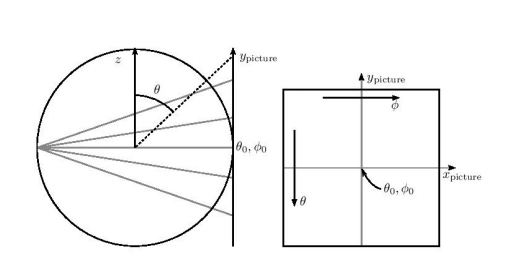
\includegraphics[width = 12.6cm, height = 8cm]{"C:/Users/Torstein/Documents/UiO/Ast2000/Python programmer"/mapping.png}
\caption{photo som viser hvordan sterografisk projeksjon fungerer, vinklene rundt en halvkule, i henholdsvis x, y og z retning, blir avstander i planet.}
\end{figure}
Det er nemlig dette projeksjonen går ut på. Vi samler inn en masse data for å lage et 360 graders bilde av himmelen og lager en stor liste med rgb verdier slik at vi kan vite i hvilken vinkel sattelitten senere peker når den selv tar et bilde.

for å sammenlikne et eventuelt bilde vi skulle ta med en 360 graders sette vi har kan vi bruke en minste kvadraters metode og rett og slett bare gå igjennom alle de 360 graders bildene, trekke alle pikslenes rgb-verdier fra pikslene i bilde vi har tatt, opphøye dem i annen og legge dem sammen, den som gir den minste summen vil da være det bilde, og dermed den retningen, som passer best til bildet vi tok.

Når vi skal finne hastigheten vår i to retninger i forhold til Stella må vi velge oss to referansestjerner. Deretter måler vi doplereffekten disse ahr når vi står i ro i forhold til Stella. Så finner vi vinkelen mellom Stella, refferansestjernene og oss, og til slutt bruker vi uttrykket $$v = \frac{A \vec{v_r}}{\sin(\phi_2 - \phi_1)}$$ der 
\begin{equation*}
A = \left[
	\begin{tabular}{ cc }
$\sin(\phi_2)$ &$ - \sin(\phi_1) $\\
$- \cos(\phi_2) $& $\cos(\phi_1)$
	\end{tabular}\right]
\end{equation*}
$\vec{v_r}$ er hastighetene i retningene til referansestjernene, funnet ved hjelp av $$\vec{v_r} = d\lambda_{ref} - d\lambda_{målt}/\lambda \cdot c$$ og $\phi_1, \phi_2$ er de to vinklene mellom refferansestjernene, sattelitten og Stella. \cite{part4}

	\section{Resultater}
		\subsection{Simulere rakett}
Når jeg simulerer boksen får jeg at antall partikler som går ut av boksen i løpet av ett sekund er ca. $7.607 \cdot 10^{13}$. På samme måte får jeg også at endringen i bevegelsesmengde som raketten blir oppnår i løpet av ett sekund er $1.19705406766 \cdot 10^{-9}$.
Fra simuleringen av utskytningen får jeg at det trengs $49000 kg$ drivstoff å få en satelitt med massen $51100$ $kg$ opp fra bakken og ut i rommet.
Med disse verdiene får jeg også at en rakett med masse på $1000$ $kg$ vil bruke $403$ $kg$ drivstoff og $3$ $sek$ på å oppnå en hastighetsendring på $1000$ $m/s$.
Til slutt får jeg også at sattelitten vil ende opp med posisjonen $(3.50933554 6.219e-05)$ $AU$ i henholdsvis x og y retning i stellas koordinatsystem, der satelitten starter med posisjon $(3.50927739, 0)$ $AU$ 

		\subsection{Simulere planetbaner}
\begin{figure}[H]
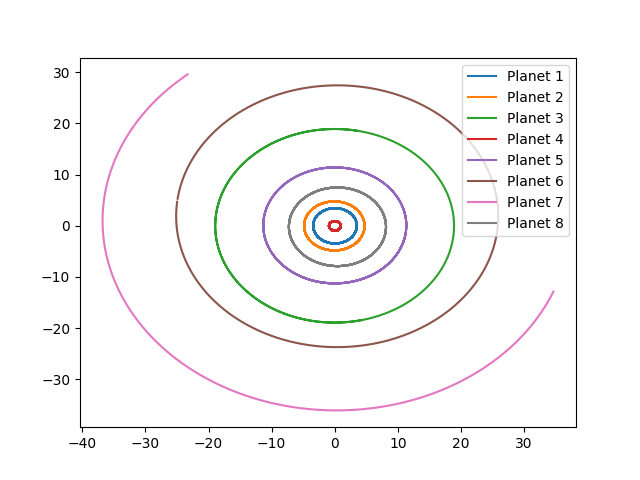
\includegraphics[width = 12.6cm, height = 8cm]{"C:/Users/Torstein/Documents/UiO/Ast2000/Python programmer"/Planetbaner.png}
\caption{Plott av banene til planetene i Stellasystemet gjennom 20 år}
\end{figure}

I prossessen ved å sjekke om stellasystemet vårt kan oppdages av andre romvesner som ser etter liv langt fant jeg disse banene for en planet, Stella og massesenteret til systemet

\begin{figure}[H]
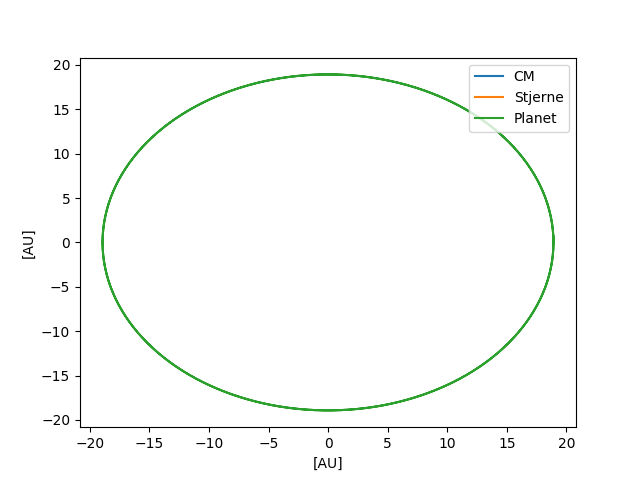
\includegraphics[width = 12.6cm, height = 8cm]{"C:/Users/Torstein/Documents/UiO/Ast2000/Python programmer"/Baner.png}
\caption{Plott av banene til planet nr. 2, hvis både planeten og Stella påvirker hverandre}
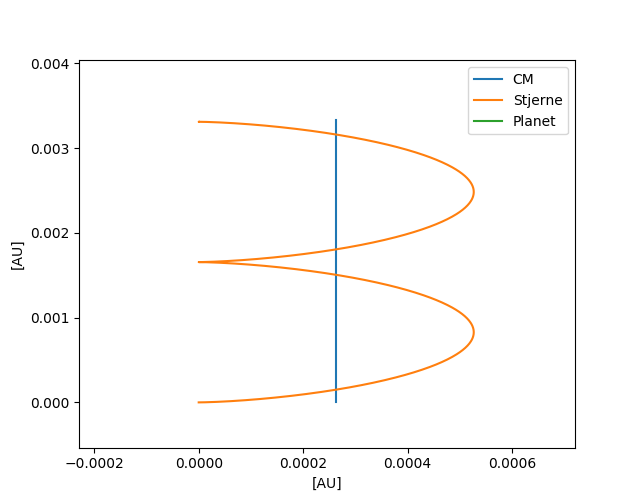
\includegraphics[width = 12.6cm, height = 8cm]{"C:/Users/Torstein/Documents/UiO/Ast2000/Python programmer"/Baner_Stella.png}
\caption{Plott av banen til massesenteret og Stella, når de blir påvirket kun av planet nr. 2}
\end{figure}

I tillegg får jeg at dette plottet av hastigheten til Stella i en spesifikk retning plottet mot tid

\begin{figure}[H]
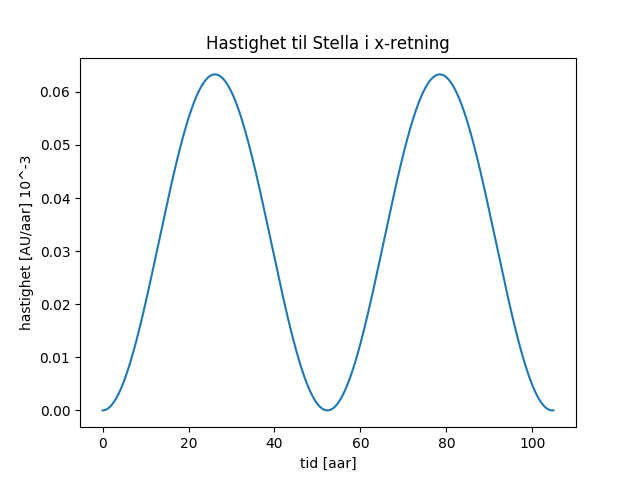
\includegraphics[width = 12.6cm, height = 8cm]{"C:/Users/Torstein/Documents/UiO/Ast2000/Python programmer"/Solhastighet.png}
\caption{Plott av hastigheten til Stella over tid}
\end{figure}

og med støy

\begin{figure}[H]
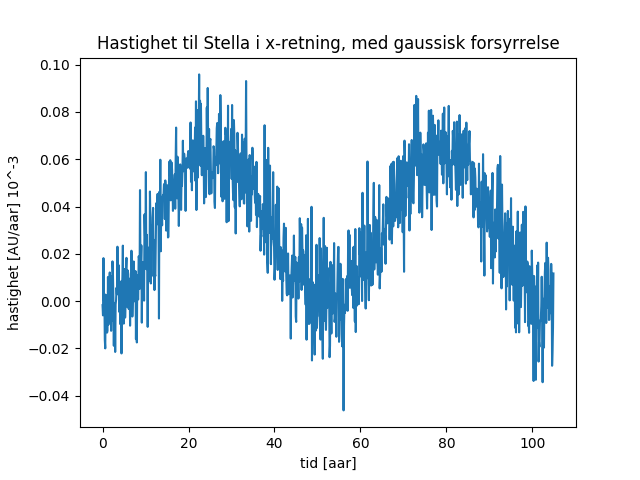
\includegraphics[width = 12.6cm, height = 8cm]{"C:/Users/Torstein/Documents/UiO/Ast2000/Python programmer"/Solhastighet_forstyrring.png}
\caption{Plott av hastigheten til Stella over tid med gaussisk støy}
\end{figure}

Den totale energien ved $10$ gjevnt fordelte tidspunkter får jeg til å bli
\begin{center}
	\begin{tabular}{| c|c |}
\hline
tid & Energi \\
\hline &  \\
0 & -0.00017837 \\
10 000 & -0.00017835 \\
20 000 & -0.00017826 \\
30 000 & -0.00017824 \\
40 000 & -0.0001783  \\
50 000 & -0.00017837 \\
60 000 & -0.00017834 \\
70 000 & -0.00017826 \\
80 000 & -0.00017824 \\
90 000 & -0.00017831 \\
\hline
	\end{tabular}
\end{center}

Til slutt finner jeg massen til planeten vår like $5.7056e-05$ $solmasser$, og at differansen til den massen vi har målt ved andre mer nøyaktige måter er $2.25665134698e-05$ $solmasser$ som vil si at jeg har fått nesten en fjerdedel mer enn jeg skulle hatt fra modellen min

		\subsection{Finne bane til satelitten}
Jeg fant ut at arealet av stellacellepanelet mitt måtte være $0.6$ $m^2$ for at det skulle være tilstrekkelig. Overflatetemperaturen på Josskro er $260.5$ grader, som er akkurat innenfor den beboelige sonen, og grensa for at en planet skal ligge innenfor den beboelige sonen er at den må ligge mellom $1.18 \cdot 10^12$ $m$ og $5.2 \cdot 10^11$ $m$ unna Stella

Fikk aldri til at denne metoden jeg brukte førte frem, viser seg at utgangshastigheten min er noe stor kanskje eller så er det noe rart i programmet som gjør at raketten ikke blir påvirket nok av kreftene fra de forskjellige objektene i stellasystemet vårt til at den endrer noe retning.
Satelitten ender bare med å skyte av gåre i en retning og ikke bry seg om noe jeg har gjordt


	\section{Diskusjon og konklusjon}
		\subsection{Simulere rakett}
De resultatene jeg fikk fra simulasjonene av boksen virket greie, og virker som de kan brukes til det jeg vil.
Jeg har laget en model av en rakett med beregninger som virker som de kan stemme. De er noe forenklet ved at vi ikke tar hensyn til atmosfærens påvirkning på raketten under oppskytning og heller ikke noen av de andre planetenes, eller stjernas påvirkning på raketten.

		\subsection{Simulere planetbaner}
Banene til planetene er ganske bra, de har form som en ellipse, noe som er riktig når vi utelikkende tar hensyn til gravitasjonskraften fra Stella. Modellen for beregningen av massen til planeten vår viser seg å ikke være så veldig nøyaktig, i og med at jeg får en feil på ca. $25 \%$, men er i hvertfall i riktig størrelsesorden, så er ikke så feil da i hvert fall.
Model for planetbanene til solsystemet, som er ganske forenklet i forhold til virkeligheten. Den tar ikke hensyn de forskjellige planetenes påvirkning på hverandre eller Stella. Modelen vil derfor antageligvis bli mer og mer unøyaktig etter som tiden går, men vil gi en helt ok bakgrunn for å beregne ruta til vår valgte planet, så lenge vi ikke venter for lenge. Modelen for to-masse systemet vil antagelig være tilstrekkelig for å merke at det er et stellasystem med planeter.

		\subsection{Finne bane til sattelitten}
Resultatene fra de første beregningene virket ganske plausible, blandt annet siden de også, selv om dette ikke ble nevt over, viste at vi også lå i den beboelige sonen.
Måten min å finne en rute fra oss til Jesskro er det derimot noe galt med, som kan skylles hvordan jeg valgte å bruke resultatene fra oppskytningen som jeg simulerte tidligere.

\addcontentsline{toc}{chapter}{Bibliography}
	\begin{thebibliography}{9}
		\bibitem{part1}
Frode Kristian Hansen; \\
1 Particles in a box \\
\texttt{http://www.uio.no/studier/emner/matnat/astro/AST2000/h17/ \\ undervisningsmateriale-2017/prosjektarbeid/part1/part1\_2017\_v2.pdf}

		\bibitem{Sciencetopia}
Terence Dangol; \\
Escape Velocity, it's Formula and Derivation \\
\texttt{https://www.sciencetopia.net/physics/escape-velocity}
		
		\bibitem{part2}
Frode Kristian Hansen; \\
Part 2: Calculating planetary orbits \\
\texttt{http://www.uio.no/studier/emner/matnat/astro/AST2000/h17/ \\
undervisningsmateriale-2017/prosjektarbeid/part2\_2017.pdf}
		
		\bibitem{Two-body problem}
Two-body problem \\
\texttt{https://en.wikipedia.org/wiki/Two-body\_problem}
		
		\bibitem{SoftSchools}
Potential Energy: Two-Body Gravitation Formula \\
\texttt{http://www.softschools.com/formulas/physics/\\
potential\_energy\_twobody\_gravitation\_formula/36/}

		\bibitem{1C}
Frode Kristian Hansen; \\
AST2000 Lecture Notes Part 1C Extrasolar planets \\
\texttt{http://www.uio.no/studier/emner/matnat/astro/AST2000/h17/ \\ undervisningsmateriale-2017/forelesningsnotater/part1c.pdf}

		\bibitem{1D}
Frode Kristian Hansen; \\
AST2000 Lecture Notes Part 1D Electromagnetic radiation
\texttt{http://www.uio.no/studier/emner/matnat/astro/AST2000/h17 \\ /undervisningsmateriale-2017/forelesningsnotater/part1d.pdf}
		\bibitem{part4}
Frode Kristian Hansen
\texttt{http://www.uio.no/studier/emner/matnat/astro/AST2000/h17/\\undervisningsmateriale-2017/prosjektarbeid/part4/part4\_2017.pdf}
	\end{thebibliography}
\end{document}